\documentclass[tikz,border=7pt]{standalone}
\usepackage{amsmath}
\usepackage{pgfplots}
\pgfplotsset{compat=1.18}
\definecolor{ink}{HTML}{17324D}
\definecolor{accent}{HTML}{0F766E}
\definecolor{gold}{HTML}{C28524}
\definecolor{violet}{HTML}{6D4AA2}
\begin{document}
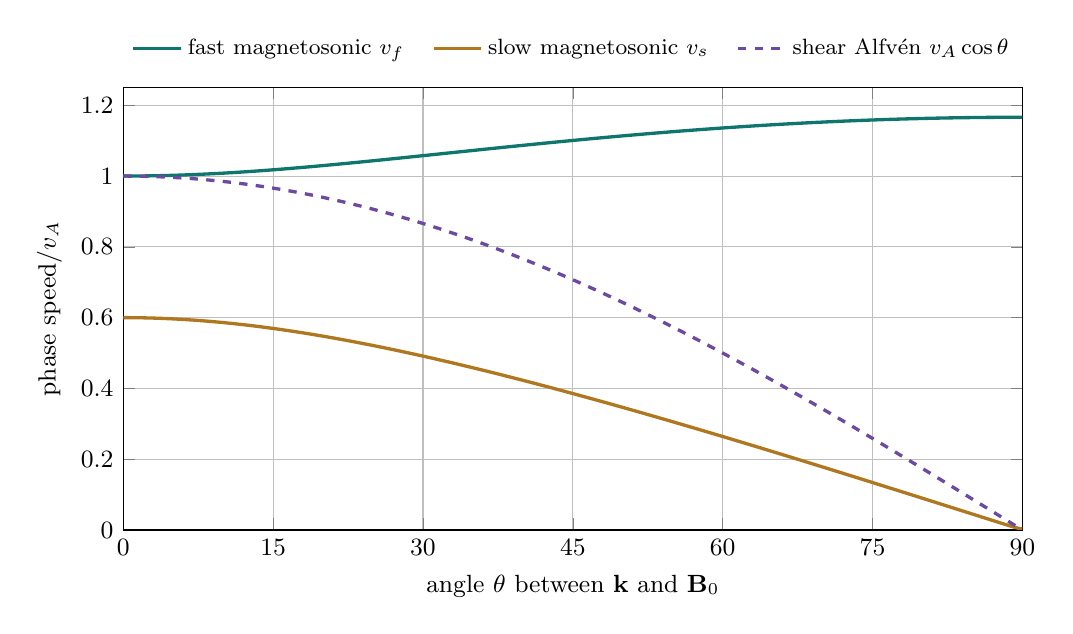
\begin{tikzpicture}
\begin{axis}[
 width=13cm,height=7.2cm,
 xmin=0,xmax=90,ymin=0,ymax=1.25,
 xlabel={angle $\theta$ between $\mathbf k$ and $\mathbf B_0$},
 ylabel={phase speed$/v_A$},
 xtick={0,15,...,90},grid=both,
 legend style={draw=none,fill=none,at={(.5,1.04)},anchor=south,
   legend columns=3,font=\footnotesize,/tikz/every even column/.append style={column sep=8pt}},
 tick label style={font=\small},label style={font=\small},
]
 \addplot[accent,very thick,domain=0:90,samples=361]
 {sqrt(.5*(1.36+sqrt(1.36^2-1.44*cos(x)^2)))};
 \addlegendentry{fast magnetosonic $v_f$}
 \addplot[gold!90!black,very thick,domain=0:90,samples=361]
 {sqrt(.5*(1.36-sqrt(1.36^2-1.44*cos(x)^2)))};
 \addlegendentry{slow magnetosonic $v_s$}
 \addplot[violet,very thick,dashed,domain=0:90,samples=361]{cos(x)};
 \addlegendentry{shear Alfv\'en $v_A\cos\theta$}
\end{axis}
\end{tikzpicture}
\end{document}
